\begin{frame}{Setup for this meeting}
\begin{itemize}
\itemsep1em
\item
Please find all material for the "hands on" sessions at:

{\color{DarkBlue}
\url{https://github.com/octave-de/octave_slides/releases/tag/2019-12-24}
}

\item
In general \textbf{Jupyter notebooks} are provided to the audience
to investigate several use cases of GNU Octave.

\item
For the best experience of the "hands on" sessions,
please bring your own laptop with Internet connection and the following setup
({\color{red}
\href{https://github.com/octave-de/octave_slides/releases/tag/2019-12-24}{setup.pdf}} at GitHub):

\begin{itemize}
\itemsep1em
\item
GNU Octave (see next slide)
\item
JupyterLab
({\color{DarkBlue}\url{https://jupyterlab.readthedocs.io/en/stable/}})
\item
octave\_kernel
({\color{DarkBlue}\url{https://github.com/Calysto/octave_kernel}})
\end{itemize}
\end{itemize}
\end{frame}


\begin{frame}{General installation steps on several systems}
$\rightarrow$ \url{https://wiki.octave.org/Installation}
\bigskip
\begin{columns}
\begin{column}{0.4\textwidth}
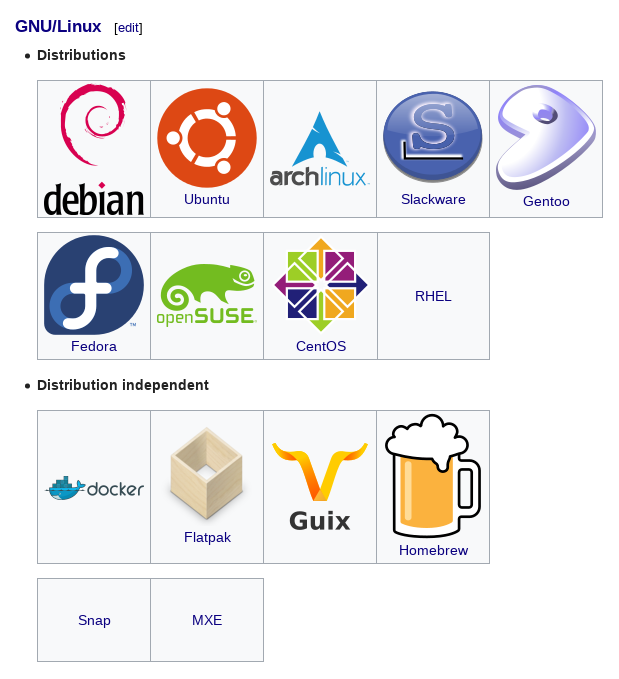
\includegraphics[width=\textwidth]{res/images/octave_wiki_install_linux}
\end{column}
\begin{column}{0.4\textwidth}
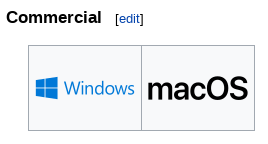
\includegraphics[width=0.42\textwidth]{res/images/octave_wiki_install_commercial}

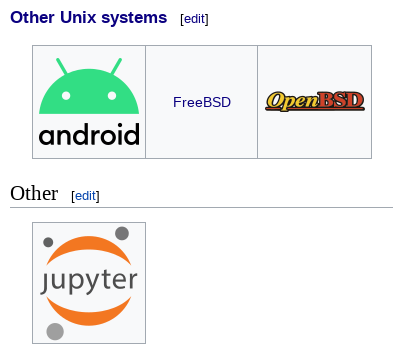
\includegraphics[width=0.6\textwidth]{res/images/octave_wiki_install_other}
\bigskip\bigskip\bigskip
\end{column}
\end{columns}
\end{frame}